\documentclass[pdflatex,a4paper]{article}

\usepackage{pgffor, ifthen}
\newcommand{\notes}[3][\empty]{%
    \noindent \vspace{10pt}\\
    \foreach \n in {1,...,#2}{%
        \ifthenelse{\equal{#1}{\empty}}
            {\rule{#3}{0.5pt}\\}
            {\rule{#3}{0.5pt}\vspace{#1}\\}
        }
}

\usepackage{graphicx}
\usepackage{xcolor}

\usepackage[margin=3cm]{geometry}

\title{Practical 12. Advanced modelling with Copasi and Python}

\author{MI Stefan}

\date{IBI1, 2018/19}


\usepackage{url}
\usepackage{amsmath}

\usepackage{listings}
\lstset{language=python}


\begin{document}

\newcommand{\<}{\textless}
\renewcommand{\>}{\textgreater}


\maketitle

\section{Introduction}

In this Practical, we will look at using Python to interact more powerfully with Copasi models. As an example, we are re-visiting the predator-prey model from the ICMB1 Copasi Practical. If you recall, the model produced oscillations for some parameter configurations. Re-familiarise yourself with the model reactions to refresh your memory. The model file is provided as an .xml file on GitHub: \verb=predator-prey.xml=

Please make sure you have committed changes for your previous practical before pulling the new files from GitHub.

\textcolor{blue}{This practical is a bit difficult. Not because it uses new skills - most of the techniques you need, you have already learned. But because the code is a bit long and it will take some concentration and tinkering around to get it right. Stay with it - you learn more by thinking about the problem for half an hour than by looking online for someone else's code. Since this practical is both difficult and close to your portfolio deadline, we are not expecting completion for your portfolio. Go as far as you can, and show us how you think by planning your steps using pseudocode. But you can get \(100\%\) on this week's assignment without having completed all of the code.}




\section{Learning objectives}


\begin{itemize}
\item
Conceptualise a biological problem into a computational model and perform simulations to address the problem
\item
Use Python to run and interpret Biochemical Models defined in COPASI
\item
Manipulate .xml files using python
\end{itemize}

\section{Running a Copasi model from within Python}

\begin{itemize}

\item
First, let's see if you can run a Copasi model from within Python. In order to do that, we start by importing a useful library: \verb=os= allows you to access your operating system from within python

\begin{lstlisting}
import os
\end{lstlisting}

\item

We have provided an .xml file for you:  \verb=predator-prey.xml= - this is an SBML version of a model that is very similar to the one you made in ICMB1, week 1.   

\item 
Download \verb=predator-prey.xml=  In order to make things simpler, make sure all your files for this practical are in the same directory. And let's also make python change into that directory. That way, your input and output file paths are nice and easy. You can set the directory using \verb=os.chdir()= 

To see whether it worked, type \verb=pwd= into your python console. This will show you the current working directory. 

\item

The command line version of Copasi is called CopasiSE. It should already be installed on your computer as part of the normal Copasi installation. Unfortunately, CopasiSE cannot easily run SBML models directly, and even in order to run .cps file, a little bit of preparation is necessary. This is achieved by the function \verb=xml_to_cps.py=, which is provided on GitHub, together with two smaller .xml files.  The code for this is a bit cumbersome and rather boring. You can treat it as a ``black box'' - just use the function and don't worry about what's in it. (This is why we have provided the function for you). 

The only part where you may have to make a change is in the command converting xml to cps (line 14): If you are using Linux or Mac, you will have to provide the path to where CopasiSE is installed. (You can probably find this using the Search function on your file system). It will look something like this:

\begin{lstlisting}
    os.system("/path/to/CopasiSE -i predator-prey.xml -s predator-prey.cps")
\end{lstlisting}

(Replace ``\verb=/path/to/CopasiSE='' by the actual path to your CopasiSE file.)

On a Windows system, you should be able to just call \verb=CopasiSE.exe= wihtout specifying the full path: 

\begin{lstlisting}
    os.system("CopasiSE.exe -i predator-prey.xml -s predator-prey.cps")
\end{lstlisting}

You are now ready to run the \verb=xml_to_cps()= function. Using this function, you should be able to convert the .xml file into a .cps file in the same directory. Check that this works as expected.

\item

Before we go on in Python, let's see whether you can run Copasi from the command line. For Linux or Mac, open a Terminal, navigate to the directory where the files for this practical are stored, and type

\begin{lstlisting}
/path/to/CopasiSE predator-prey.cps
\end{lstlisting}

For Windows, open Git Bash, navigate to the directory where the files for this practical are stored, and type

\begin{lstlisting}
CopasiSE.exe predator-prey.cps
\end{lstlisting}


\item
How can you see whether it works? Copasi should have created a new file for you, \verb=model_results.csv= (csv stands for ``comma separated values'' - this is a file that contains your results. Each line corresponds to a time point, and values of time, A, and B at each time point are listed, separated by commas. The first line just contains all variable names. You can have a look at the file in a text editor if you want.)

\item
Now that we can do it within the command line, let's do it outside the command line, from Python! The command you need for that is \verb=os.system()= Within the parentheses, use quotes and type whatever it is you would otherwise type into your command line. Here, for instance, we need 

\begin{lstlisting}
os.system(``/path/to/CopasiSE predator-prey.cps'')
\end{lstlisting}

or 

\begin{lstlisting}
os.system(``CopasiSE.exe predator-prey.cps'')
\end{lstlisting}

\emph{How can you tell whether this worked?}

\end{itemize}

\section{Reading and plotting simulation results}

\begin{itemize}
\item
OK, so the output of our model is stored as comma-separated values in file \verb=modelResults.csv= (An example of such a file is also provided in your GitHub repository). Do you remember how to read the content of a file into Python?
\item
It is probably useful to make two arrays: One called ``names'' that just contains the variable names (i.e. the first line of your Results file), and another one which contains the results data. (This will be an array of arrays, one for each time point). Can you make those using the data from your results file? You may find the \verb=split()= function useful: It splits the content of a line into separate entries in an array, using a user-defined separator. For instance, if you have 

\begin{lstlisting}
line = ``1, 2, 3, 4, 5''
\end{lstlisting}

Then \verb=line.split(",")= will give you \verb=['1', '2', '3', '4', '5']=

\item
As we said earlier, your array of results will have a row for each time point and a column for each variable. If you transform it into a numpy array, this makes indexing easier. For this, you have to first import numpy. If your results array is called \verb=results=, the command to transform it is 

\begin{lstlisting}
results = numpy.array(results)
\end{lstlisting}

Also using numpy, let's transform the numbers into actual numbers (at the moment, Python thinks they are strings)

\begin{lstlisting}
results = results.astype(numpy.float)
\end{lstlisting}



The beauty of a numpy array is that its elements can be accessed using \verb=arrayname[x,y]= where x and y stand for the x and y coordinate. For instance, if you want to see the content of row 0 and column 1 of \verb=results=, the command for that is 

\begin{lstlisting}
results[0,1]
\end{lstlisting}

If you want to see a range of coordinates, use the colon, for instance: 

\begin{lstlisting}
results[0:3,1]
\end{lstlisting}

or

\begin{lstlisting}
results[0,:]
\end{lstlisting}

\item

You now know enough to make some nice plots. First, plot a time course of the predator and prey population. It should look something like this:

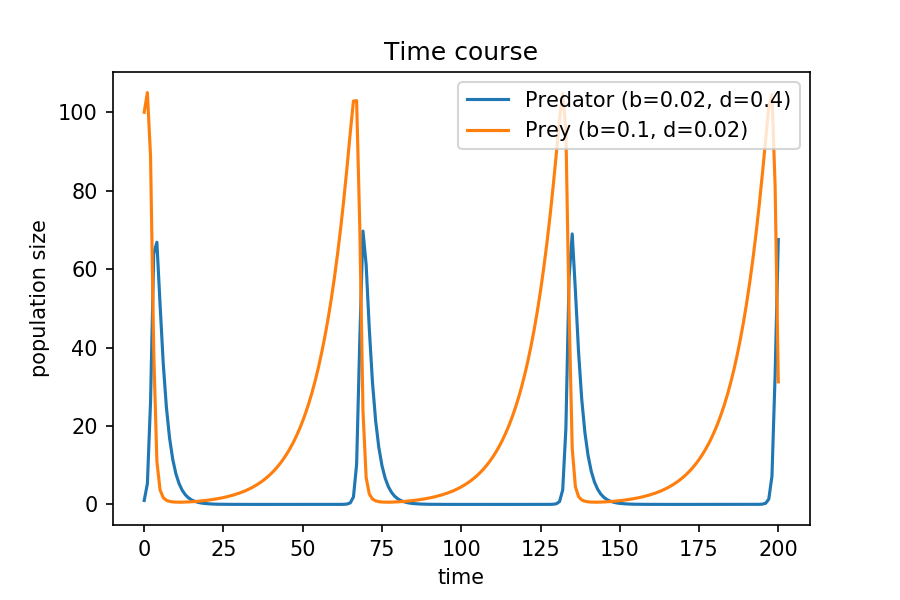
\includegraphics{time_course0.png}

\item

Second, let's make a plot that's a bit more complicated: A limit cycle plot. Instead of plotting populations against time, this plots predator population against prey population. (\emph{Why would this be useful or interesting?})

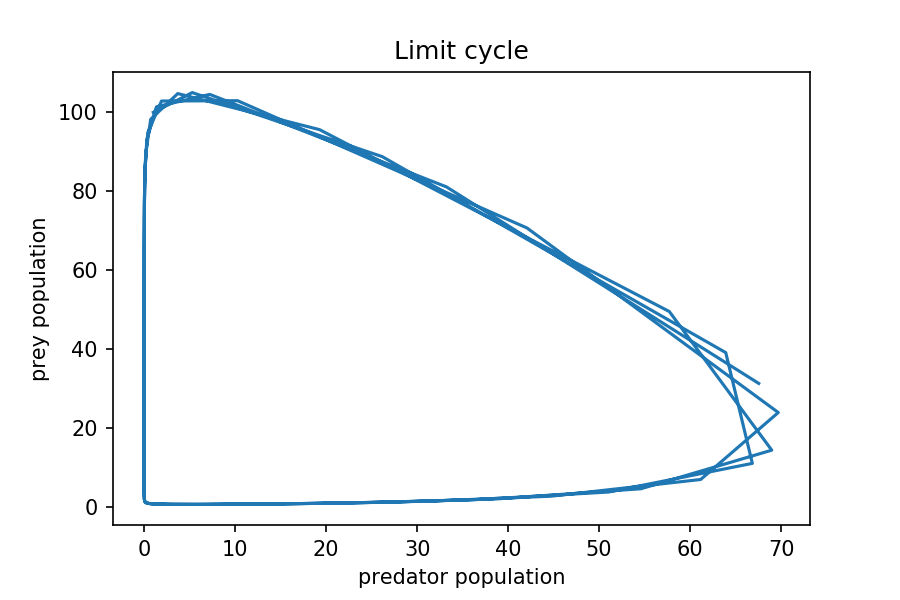
\includegraphics{limit_cycle0.png}

\end{itemize}


\section{Changing values and running the simulation again}

\begin{itemize}
\item
So far so good - and this should be similar to what you saw when you ran the model in Copasi as well. Now for the interesting part: How much does what you see depend on the particular parameters of your model? For this exercise, we will look at the four rate parameters, that govern birth and death of the predator and prey, respectively. In our model, those are called  k\_predator\_breeds, k\_predator\_dies, k\_prey\_breeds, k\_prey\_dies,  respectively. Pick a number (any number) between 0 and 1 for each of them. 
\item
Recall that SBML is just fancy xml. You can use python to edit an SBML file the same way as any other .xml file. Do you remember how to read the file into python, see and change parameters, and save the file again? Refer to your notes from week 8 if you are confused. The \verb=dom.minidom= package will come in handy.
\item
Once you have changed the values, run the simulation again. Do you see a difference? Here is an example from one of our models (but yours will probably look quite different).

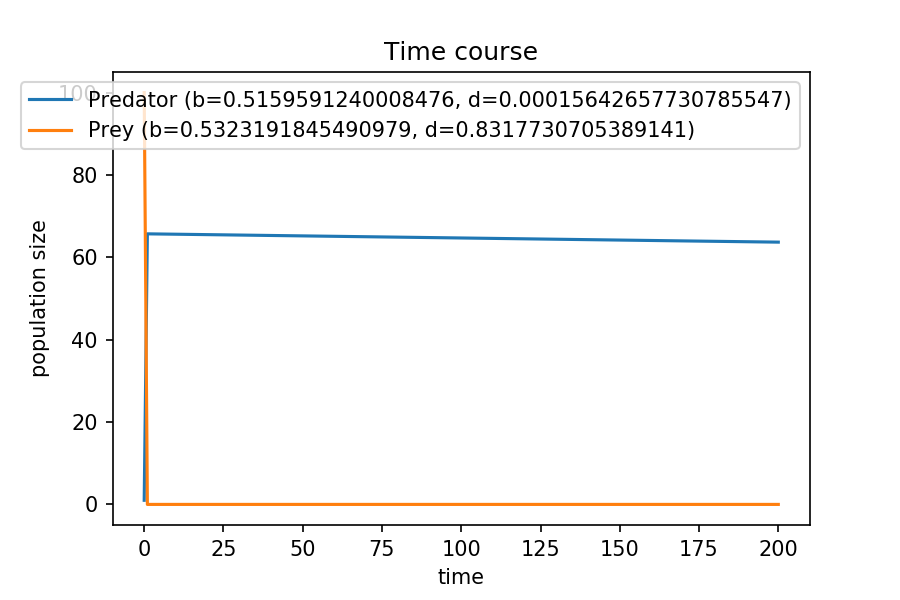
\includegraphics{time_course2.png}

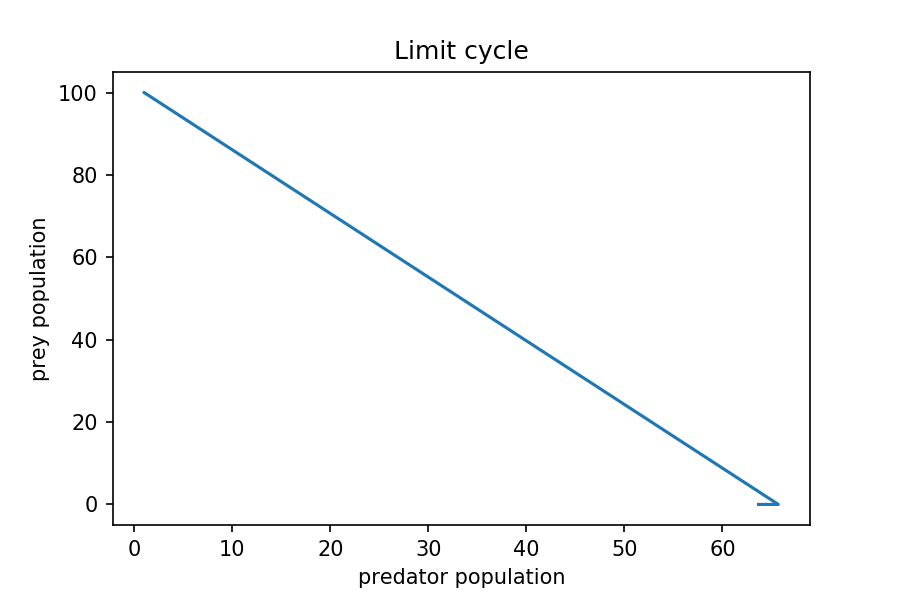
\includegraphics{limit_cycle2.png}

\end{itemize}

\section{Running many simulations}

\begin{itemize}
\item
Instead of changing parameters manually and running a simulation, can you run 100 simulations with 100 different parameter combinations? (Or more?) You may want to vary parameters systematically, or you may want to pick random numbers. In the latter case, you may find the function \verb=numpy.random.sample()= quite useful. In the absence of arguments, it will just draw a random number between 0 and 1.
\item
Think a little bit about what you would like the output to be. What we did was create a separate figure (with a slightly different name) for each of the simulations, and adding the parameter configuration to the figure legend. But you may think of other ways to keep track of the results of all your simulations - maybe you are interested in the maximum number of predators in your simulation, or in whether your prey dies out during the course of the simulation, or whether or not there are oscillations, \dots - Follow your interest and think of a good way of collecting and then showing that data. 
\end{itemize}




\section{For your portfolio}

The markers will look for and assess the following:

\begin{itemize}
\item
File runPredatorPrey.py exists
\item
You can run a Copasi file from within Python
\item
You can plot the content of a .csv file
\item
Plots are well labelled
\item
There is an attempt at altering the SBML file using xml editing functionality in Python. (It need not be perfect, or complete, but there should be an idea of how to do this, as evidenced by planning in pseudocode.)
\item
There is an attempt at running a number of simulations and somehow assessing the results - visually or otherwise. (It need not be perfect, or complete, but the idea should be sketched out in pseudocode.)
\end{itemize}



\end{document}


